 \pstart [p.~85] XVI. Vobis autem expendendum propono, annon exhinc\footnote{\textit{Gedruckte Marginalie}: Fig. 128.} \textit{apparentiarum in }\textit{Iride}\protect\index{Sachverzeichnis}{iris}\textit{ ratio} elici possit, illa forte verisimilior, quam\footnote{\textit{Leibniz unterstreicht}: illa [...] quam} ipse \textit{Cartesius}\protect\index{Namensregister}{\textso{Descartes} (Cartesius, des Cartes, Cartes.), Ren\'{e} 1596\textendash 1650} assignavit.
 \pend
   \begin{center}
   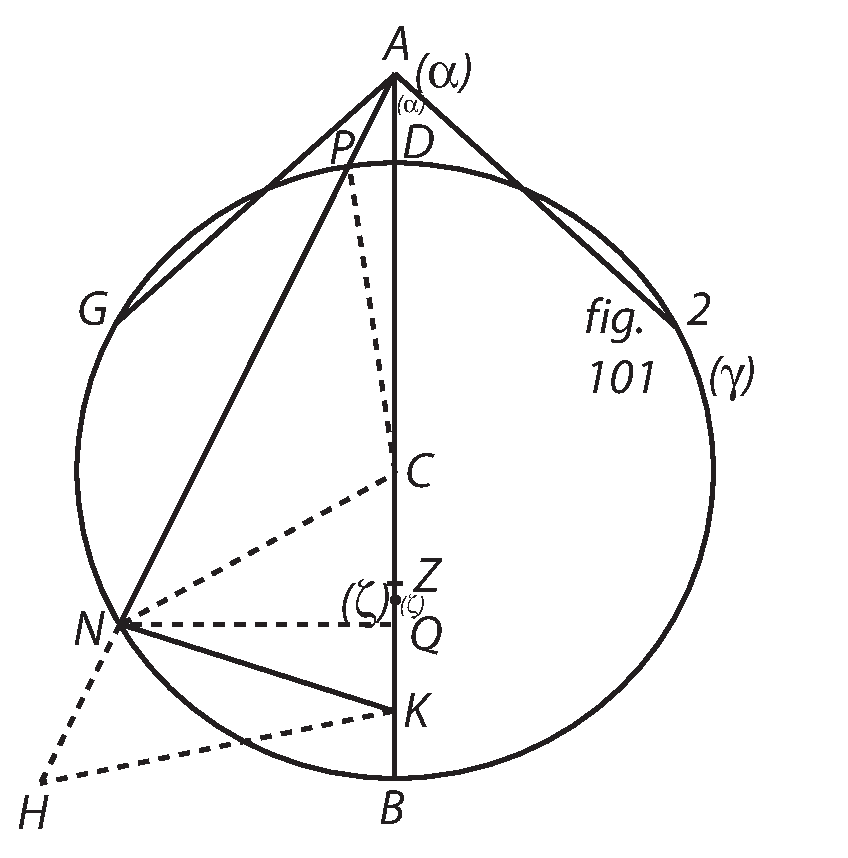
\includegraphics[width=0.4\textwidth]{images/T8_Barrow-2}
   \\ \textit{[Fig. 2]}\footnote{\textit{Unterhalb von fig. 101}:  \renewcommand{\arraystretch}{2.0} \protect\begin{tabular}{c}$\displaystyle\frac{CZ}{CB}$ aequ. $\displaystyle\frac{AC}{AB}$\hspace{5mm}$CK$ majus $CZ$\end{tabular}}\end{center}
\clearpage
   \begin{center} \vspace{2.0ex}
   \includegraphics[width=0.3\textwidth]{images/T8_Barrow-1}
   \\ \textit{[Fig. 1]}\footnote{\textit{Oberhalb von fig. 97:} \textit{AN} aequ. \textit{AC}}
   \end{center}